%!TEX root = thesis.tex

\chapter{Follow-Up User Study}
\label{chap:follow-up-user-study}

A follow-up user study was conducted to evaluate the set of refined visualisations (see Chapter~\ref{chap:visualisation-refinement}) and to address some of the limitations identified in the first user study. This included providing a valid baseline for the study (the \emph{no visualisation} condition) and reducing the visualisations to more meaningful representations.

It was hypothesised that the visualisation prototype would result in higher understanding at the end of the performance and that enjoyment would remain steady throughout both performances.

\section{Method}

Two independent audiences ($N=14+11=25$) were recruited through on campus advertisement (see Appendix~\ref{appendix:follow-up-user-study-advertisement}). Each group was exposed to two live coding musical performances. One of the performances displayed only the source code of the performance while the other displayed the source code with the refined visualisation prototype as an underlay (see Chapter~\ref{chap:visualisation-refinement}).

The first group was subjected to the \emph{visualisation} condition, followed by the \emph{no visualisation} condition. The conditions were swapped for the second group, with the audience exposed to the \emph{no visualisation} condition first followed by the \emph{visualisation} condition.

Again, over the course of these performances, each audience member completed a survey consisting of four sections: demographic information, their opinion of the first piece, their opinion of the second piece and questions about the performance overall. 

Two additional questions were asked to get an impression of the audience's understanding at specific stages of the performance: ``What do you think the performer was doing in the very early stages of the performance?'' and ``What do you think the performer was doing in the very last stages of the performance?''. The results of these questions would then be compared to the reported levels of understanding through the performance to evaluate the accuracy of the measure.

\section{Participants}

Of the 25 total participants over the two performances $12\%$ were female. $64\%$ of the audience had not been to a live coding performance before and $80\%$ had not attended the previous live coding user study. The background of the audience included $56\%$ that listened to music regularly, $28\%$ that played an instrument and $72\%$ who programmed for their hobby, job or study.

\section{Results}

\begin{figure}
  \centering
  \includegraphics[width=\columnwidth]{../study-3/results/dimension-condition-study-3.pdf}
  \caption[Follow-up user study survey condition and dimension results]{Percentage of the audience reporting ``high'' (green - above the line) and ``low'' (red - below the line) enjoyment and understanding over the beginning, middle and end stages of the performances for the no visualisation and visualisation conditions. The remaining population, not shown here, reported ``medium'' levels of enjoyment or understanding.}
  \label{fig:dimension-condition-follow-up-user-study}
\end{figure}

The audience-reported enjoyment and understanding responses from the survey were evaluated for the two conditions as described below. A summary of the results can be seen in Figure~\ref{fig:dimension-condition-follow-up-user-study}.

\subsection{Enjoyment}

\begin{figure}
\centering
\begin{subfigure}{\textwidth}
  \centering
  \includegraphics[width=\columnwidth,page=7]{../images/graphs/condition-dimension.pdf}
  \caption[No visualisation condition enjoyment detailed survey results]{Audience reported enjoyment level for the \textbf{no visualisation} condition.}
  \label{fig:no-visualisation-enjoyment}
\end{subfigure}\\
\begin{subfigure}{\textwidth}
  \centering
  \includegraphics[width=\columnwidth,page=8]{../images/graphs/condition-dimension.pdf}
  \caption[Visualisation condition enjoyment detailed survey results]{Audience-reported enjoyment level for the \textbf{visualisation} condition.}
  \label{fig:visualisation-enjoyment}
\end{subfigure}

\caption[Follow-up user study enjoyment survey responses]{Audience reported enjoyment during the beginning, middle and end of the performance for the no visualisation and visualisation conditions. Line width at each stage indicates proportion of the audience reporting high, medium or low enjoyment, and line colour connecting each section of the performance is determined by the enjoyment level at the \emph{beginning} of the performance.}
\label{fig:follow-up-user-study-condition-enjoyment}
\end{figure}

Audiences were asked to state if they thought the source code projection helped their enjoyment of the performance and if they thought the visualisations helped their enjoyment of the performance. $60\%$ of the audience stated that projection of the source code helped their enjoyment of the performance directly while $16\%$ stated that the visualisations helped their enjoyment directly.

Levels of enjoyment throughout the performance were surveyed for the \emph{beginning}, \emph{middle} and the \emph{end} phases of the performance. A comparison of the enjoyment between the no visualisation condition and the visualisation condition is available in Figure~\ref{fig:no-visualisation-enjoyment} and Figure~\ref{fig:visualisation-enjoyment}.

Final levels of enjoyment between the two conditions differed only slightly. With no visualisation, $20\%$ stated that they had low enjoyment, $40\%$ stated that they had medium enjoyment and $40\%$ stated that they had high enjoyment. With visualisations, $20\%$ stated low enjoyment, $36\%$ stated medium enjoyment and $44\%$ stated high enjoyment.

\subsection{Understanding}

\begin{figure}
\centering
\begin{subfigure}{\textwidth}
  \centering
  \includegraphics[width=\columnwidth,page=5]{../images/graphs/condition-dimension.pdf}
  \caption[No visualisation condition understanding detailed survey results]{Audience reported understanding level for the \textbf{no visualisation} condition.}
  \label{fig:no-visualisation-understanding}
\end{subfigure}\\
\vspace{15mm}
\begin{subfigure}{\textwidth}
  \centering
  \includegraphics[width=\columnwidth,page=6]{../images/graphs/condition-dimension.pdf}
  \caption[Visualisation condition understanding detailed survey results]{Audience-reported understanding level for the \textbf{visualisation} condition.}
  \label{fig:visualisation-understanding}
\end{subfigure}
\vspace{15mm}
\caption[Follow-up user study understanding survey responses]{Audience reported understanding during the beginning, middle and end of the performance for the no visualisation and visualisation conditions. Line width at each stage indicates proportion of the audience reporting high, medium or low understanding, and line colour connecting each section of the performance is determined by the understanding level at the \emph{beginning} of the performance.}
\label{fig:follow-up-user-study-condition-understanding}
\end{figure}

Audiences were asked to state if they thought the source code projection helped their understanding of the performance and if they thought the visualisations helped their understanding of the performance. Of the audience, $76\%$ stated that projection of the code helped their understanding of the performance directly while $32\%$ stated that the visualisations helped their understanding directly.

Levels of understanding throughout the performance were surveyed for the \emph{beginning}, \emph{middle} and the \emph{end} phases of the performance. A comparison of the understanding between the no visualisation condition and the visualisation condition is available in Figure~\ref{fig:no-visualisation-understanding} and Figure~\ref{fig:visualisation-understanding}.

Levels of understanding also differed slightly between the two conditions. With no visualisation, $32\%$ stated that they had low understanding, $48\%$ stated that they had medium understanding and $20\%$ stated that they had high understanding. With visualisations, $28\%$ stated low understanding, $44\%$ stated medium understanding and $28\%$ stated high understanding.

\subsection{Liveness}

After exposing the audience to both conditions, the audience was asked if the projected source code or visualisations helped to communicate the feeling that the performances were live. Of the twenty-five responses, eighteen indicated that the projection of the source code helped, though the audience overall was experienced in programming. 

Results of this question reflected the audience opinion of the visualisations. Some responses indicated that: ``Yes. Live code editing [helped to communicate the liveness], but visualisations showed what coder was looking at and editing as well as what was running.''. In contrast, members of the audience stated that the ``visualisations [were] not really useful, didn't seem in sync with the music and [had] no obvious meaning''. However, most of the audience ($64\%$) focussed on the source code or musical aspects of the performance in their discussion.

\section{Discussion}

Overall, only minor differences were observed between the no visualisation and visualisation conditions. Few differences in enjoyment were seen between the two conditions. Mirroring the previous user study, a pattern of lower understanding was seen with the visualisations during the beginning of the performance. This result supports the idea that visualisations targeting understanding take some time to understand and may only provide benefits in the long-term. 

After each performance, two additional questions asked the audience to explain what they thought the live coder was doing at the beginning of the performance and to explain what they thought the live coder was doing at the end of the performance. Results of these questions indicate that many members of the audience had a good understanding of the musical aspects of the performance. Responses stating that the live coder was ``adding instruments'' and ``setting up repetitive sequences to build on during the session'' suggested a good overall comprehension of the early stages of the performance. Similarly, when asked about the last stages of the performance, responses stating that the live coder was ``changing variables in order to add or remove instruments and alter the pace of the music'' indicate a high level of understanding and experience with programming. A number of other responses indicated that understanding was low. For example, one audience member stated: ``Sorry, I don't quite understand''. Overall, the patterns of understanding reported over the three phases of the performance match the responses asking the audience to explain their understanding.


\subsection{Comparison to Previous Study}

Both studies were conducted under similar conditions and it is reasonable that the results of the studies could be directly compared. Comparing Figure~\ref{fig:dimension-condition-follow-up-user-study} to Figure~\ref{fig:dimension-condition} reveals some interesting observations regarding the two user studies. It is immediately obvious that a larger proportion of audience members reported low understanding during the follow-up user study than the initial user study. Similar patterns are seen in the proportion of the audience reporting low enjoyment at the beginning of the performance.

The proportion of the audience reporting high levels of understanding is fairly similar across both studies with the exception of the end of the performance for the follow-up user study visualisation condition during which a larger proportion of the audience reported high understanding.

Across the aesthetic, didactic, visualisation, and no visualisation conditions, the aesthetic condition resulted in the highest levels of enjoyment. The visualisation, no visualisation and didactic conditions all performed poorly regarding understanding during the beginning of the performance.

\subsection{Limitations}

A number of factors were identified that could influence the validity of the user study results.

The visualisations suffered from being obscured by the source code displayed on the projection screen. However, compared to the initial user study, the visualisations were logically placed in relation to the source code, from top to bottom, in the order the functions appeared in the code to attempt to counteract this interference.

Nevertheless, one member of the audience stated that ``the visualisation made sense of the separate parts [of the code] so you could track each easier but [the visualisations] were difficult to see''. The difficulty in seeing the visualisations was discussed by a number of members of the audience, generally stating that the visualisations were projected too faintly behind the source code.

A large proportion of the audience stated that they had coding experience. This may have influenced the preference for seeing the source code during live coding performances. An audience experienced in coding may be less interested in viewing visualisations and have a preference for viewing code directly without anything interfering with the source code.

Finally, as with the first user study, musical and visual preference may have contributed to the results of the survey. Again, an attempt was made to mitigate this through similar musical styles through all performances.

\section{Summary}

This study identifies some small differences between live coding with and without visualisations. A larger proportion of the audience had high enjoyment during the middle of the performance when a visualisation was displayed than without. Similarly, the visualisations resulted in a small increase in the proportion of the audience reporting high understanding. However, this was offset by fewer reporting high understanding at the beginning of the performance.

Although some variation was found, the sample size limited the conclusions that could be made. A comparison with the previous user study suggested that the visualisations examined within this chapter did not quite capture the enjoyment patterns of the aesthetic visualisations. However, an increase in the proportion reporting high understanding for the visualisation condition examined in this chapter suggest that understanding may have been influenced despite the technical challenges encountered.


